\documentclass[10pt]{article}
\usepackage[margin=1in]{geometry}
\usepackage{amsmath,amssymb,booktabs,graphicx,xcolor}
\usepackage[numbers,sort&compress]{natbib}
\usepackage[hidelinks]{hyperref}
\usepackage{caption}
\captionsetup{font=small,labelfont=bf}
\newcommand{\cnncefinal}{76.5}
\newcommand{\cnncefirst}{68.7}
\newcommand{\cnncelogt}{0.35}
\newcommand{\cnncetemp}{1.42}
\newcommand{\cnncecost}{0.66}
\newcommand{\cnncecostpe}{0.61}
\newcommand{\cnncecostts}{0.72}
\newcommand{\cnnceearly}{44}
\newcommand{\cnnceprec}{21}
\newcommand{\cnncegap}{43}
\newcommand{\cnnceprects}{27}
\newcommand{\cnnceprecloco}{37}
\newcommand{\cnnceearlyloco}{13}
\newcommand{\cnnceeceraw}{58}
\newcommand{\cnnceecets}{37}
\newcommand{\cnnceeceloco}{16}
\newcommand{\cnnkdfinal}{76.1}
\newcommand{\cnnkdfirst}{70.5}
\newcommand{\cnnkdlogt}{0.46}
\newcommand{\cnnkdtemp}{1.59}
\newcommand{\cnnkdcost}{0.54}
\newcommand{\cnnkdcostpe}{0.50}
\newcommand{\cnnkdcostts}{0.61}
\newcommand{\cnnkdearly}{74}
\newcommand{\cnnkdprec}{17}
\newcommand{\cnnkdgap}{57}
\newcommand{\cnnkdprects}{21}
\newcommand{\cnnkdprecloco}{26}
\newcommand{\cnnkdearlyloco}{33}
\newcommand{\cnnkdeceraw}{62}
\newcommand{\cnnkdecets}{40}
\newcommand{\cnnkdeceloco}{18}
\newcommand{\cnnstrongfinal}{80.1}
\newcommand{\cnnstrongfirst}{66.7}
\newcommand{\cnnstronglogt}{-0.40}
\newcommand{\cnnstrongtemp}{0.67}
\newcommand{\cnnstrongcost}{1.05}
\newcommand{\cnnstrongcostpe}{0.88}
\newcommand{\cnnstrongcostts}{1.07}
\newcommand{\cnnstrongearly}{3}
\newcommand{\cnnstrongprec}{76}
\newcommand{\cnnstronggap}{9}
\newcommand{\cnnstrongprects}{74}
\newcommand{\cnnstrongprecloco}{76}
\newcommand{\cnnstrongearlyloco}{4}
\newcommand{\cnnstrongeceraw}{15}
\newcommand{\cnnstrongecets}{32}
\newcommand{\cnnstrongeceloco}{18}
\newcommand{\vitplainfinal}{59.9}
\newcommand{\vitplainfirst}{59.5}
\newcommand{\vitplainlogt}{0.97}
\newcommand{\vitplaintemp}{2.64}
\newcommand{\vitplaincost}{0.20}
\newcommand{\vitplaincostpe}{0.20}
\newcommand{\vitplaincostts}{0.29}
\newcommand{\vitplainearly}{96}
\newcommand{\vitplainprec}{15}
\newcommand{\vitplaingap}{63}
\newcommand{\vitplainprects}{20}
\newcommand{\vitplainprecloco}{22}
\newcommand{\vitplainearlyloco}{65}
\newcommand{\vitplaineceraw}{62}
\newcommand{\vitplainecets}{26}
\newcommand{\vitplaineceloco}{12}
\newcommand{\vitcefinal}{71.3}
\newcommand{\vitcefirst}{65.8}
\newcommand{\vitcelogt}{-0.31}
\newcommand{\vitcetemp}{0.74}
\newcommand{\vitcecost}{0.51}
\newcommand{\vitcecostpe}{0.43}
\newcommand{\vitcecostts}{0.49}
\newcommand{\vitceearly}{10}
\newcommand{\vitceprec}{70}
\newcommand{\vitcegap}{5}
\newcommand{\vitceprects}{67}
\newcommand{\vitceprecloco}{70}
\newcommand{\vitceearlyloco}{10}
\newcommand{\vitceeceraw}{11}
\newcommand{\vitceecets}{23}
\newcommand{\vitceeceloco}{16}
\newcommand{\vitkdfinal}{71.3}
\newcommand{\vitkdfirst}{66.4}
\newcommand{\vitkdlogt}{-0.33}
\newcommand{\vitkdtemp}{0.72}
\newcommand{\vitkdcost}{0.45}
\newcommand{\vitkdcostpe}{0.37}
\newcommand{\vitkdcostts}{0.42}
\newcommand{\vitkdearly}{18}
\newcommand{\vitkdprec}{59}
\newcommand{\vitkdgap}{3}
\newcommand{\vitkdprects}{54}
\newcommand{\vitkdprecloco}{59}
\newcommand{\vitkdearlyloco}{17}
\newcommand{\vitkdeceraw}{11}
\newcommand{\vitkdecets}{24}
\newcommand{\vitkdeceloco}{16}
\newcommand{\cnncecostloco}{--}
\newcommand{\cnnkdqfinal}{--}
\newcommand{\cnnkdqfirst}{--}
\newcommand{\cnnkdqlogt}{--}
\newcommand{\cnnkdqtemp}{--}
\newcommand{\cnnkdqcost}{--}
\newcommand{\cnnkdqcostpe}{--}
\newcommand{\cnnkdqcostts}{--}
\newcommand{\cnnkdqearly}{--}
\newcommand{\cnnkdqprec}{--}
\newcommand{\cnnkdqgap}{--}
\newcommand{\cnnkdqprects}{--}
\newcommand{\cnnkdqprecloco}{--}
\newcommand{\cnnkdqearlyloco}{--}
\newcommand{\cnnkdqeceraw}{--}
\newcommand{\cnnkdqecets}{--}
\newcommand{\cnnkdqeceloco}{--}
\newcommand{\cnnkdqcostloco}{--}
\newcommand{\cnnkdcostloco}{--}
\newcommand{\cnnkdtfinal}{--}
\newcommand{\cnnkdtfirst}{--}
\newcommand{\cnnkdtlogt}{--}
\newcommand{\cnnkdttemp}{--}
\newcommand{\cnnkdtcost}{--}
\newcommand{\cnnkdtcostpe}{--}
\newcommand{\cnnkdtcostts}{--}
\newcommand{\cnnkdtearly}{--}
\newcommand{\cnnkdtprec}{--}
\newcommand{\cnnkdtgap}{--}
\newcommand{\cnnkdtprects}{--}
\newcommand{\cnnkdtprecloco}{--}
\newcommand{\cnnkdtearlyloco}{--}
\newcommand{\cnnkdteceraw}{--}
\newcommand{\cnnkdtecets}{--}
\newcommand{\cnnkdteceloco}{--}
\newcommand{\cnnkdtcostloco}{--}
\newcommand{\cnnlsfinal}{--}
\newcommand{\cnnlsfirst}{--}
\newcommand{\cnnlslogt}{--}
\newcommand{\cnnlstemp}{--}
\newcommand{\cnnlscost}{--}
\newcommand{\cnnlscostpe}{--}
\newcommand{\cnnlscostts}{--}
\newcommand{\cnnlsearly}{--}
\newcommand{\cnnlsprec}{--}
\newcommand{\cnnlsgap}{--}
\newcommand{\cnnlsprects}{--}
\newcommand{\cnnlsprecloco}{--}
\newcommand{\cnnlsearlyloco}{--}
\newcommand{\cnnlseceraw}{--}
\newcommand{\cnnlsecets}{--}
\newcommand{\cnnlseceloco}{--}
\newcommand{\cnnlscostloco}{--}
\newcommand{\cnnmixfinal}{--}
\newcommand{\cnnmixfirst}{--}
\newcommand{\cnnmixlogt}{--}
\newcommand{\cnnmixtemp}{--}
\newcommand{\cnnmixcost}{--}
\newcommand{\cnnmixcostpe}{--}
\newcommand{\cnnmixcostts}{--}
\newcommand{\cnnmixearly}{--}
\newcommand{\cnnmixprec}{--}
\newcommand{\cnnmixgap}{--}
\newcommand{\cnnmixprects}{--}
\newcommand{\cnnmixprecloco}{--}
\newcommand{\cnnmixearlyloco}{--}
\newcommand{\cnnmixeceraw}{--}
\newcommand{\cnnmixecets}{--}
\newcommand{\cnnmixeceloco}{--}
\newcommand{\cnnmixcostloco}{--}
\newcommand{\cnnrafinal}{--}
\newcommand{\cnnrafirst}{--}
\newcommand{\cnnralogt}{--}
\newcommand{\cnnratemp}{--}
\newcommand{\cnnracost}{--}
\newcommand{\cnnracostpe}{--}
\newcommand{\cnnracostts}{--}
\newcommand{\cnnraearly}{--}
\newcommand{\cnnraprec}{--}
\newcommand{\cnnragap}{--}
\newcommand{\cnnraprects}{--}
\newcommand{\cnnraprecloco}{--}
\newcommand{\cnnraearlyloco}{--}
\newcommand{\cnnraeceraw}{--}
\newcommand{\cnnraecets}{--}
\newcommand{\cnnraeceloco}{--}
\newcommand{\cnnracostloco}{--}
\newcommand{\cnnstrongcostloco}{--}
\newcommand{\vitplaincostloco}{--}
\newcommand{\vitcecostloco}{--}
\newcommand{\vitkdcostloco}{--}
\newcommand{\nruns}{18}
\newcommand{\rhoprec}{-0.87}
\newcommand{\rhots}{0.47}
\newcommand{\minrankcorr}{0.95}
\newcommand{\basegflops}{1.11}
\newcommand{\baseacc}{76.1}
\newcommand{\speedcpu}{1.90}
\newcommand{\speedgpu}{1.06}


\title{Confident Exits Are Cheap but Brittle:\\ Training Recipes Govern Early-Exit Reliability under Distribution Shift}
\author{Aditya Goyal \and Raunak Panshikar \and Arth Mishra \and Kartikey Goyal\\
\small School of Computer Engineering, Manipal Institute of Technology, Manipal Academy of Higher Education}
\date{}

\begin{document}
\maketitle

\begin{abstract}
Early-exit networks save computation by stopping an input at the first intermediate classifier whose confidence
clears a threshold. Prior work showed that such exits lose calibration under common corruptions and stop too
early. We ask what controls this behaviour. On CIFAR-100, with early-exit ResNet-18 and ViT-Tiny models, four
distillation weights, two training recipes and their components, three seeds per configuration and 30 corruption
conditions, we find that the confidence state of the exits, which we measure by their fitted temperature, predicts
how reliable early exits remain under shift (Spearman $\rho=\rhoprec$ across \nruns{} runs), and that it is set by
the training recipe rather than the architecture. A CNN trained with label smoothing, mixup and RandAugment becomes
underconfident and lets only \cnnstrongearly\% of severely corrupted inputs exit early, \cnnstrongprec\% of them
correctly, while a ViT trained without them becomes overconfident and lets \vitplainearly\% exit early with
\vitplainprec\% accuracy. Self-distillation from the final exit, a standard way to strengthen early exits, raises
confidence: it reduces clean computation at matched validation accuracy from \cnncecost{} to \cnnkdcost{} GFLOPs but
raises the share of severely corrupted inputs that exit early from \cnnceearly\% to \cnnkdearly\%, with lower
accuracy. Temperature scaling fitted on clean data barely re-ranks predictions (rank correlation $\geq\minrankcorr$)
and is dominated by per-exit thresholds; temperatures fitted on held-out corruption types cut the final-exit
calibration error of the distilled CNN at severity 5 from \cnnkdecets\% to \cnnkdeceloco\% and raise early-exit
accuracy from \cnnkdprects\% to \cnnkdprecloco\%. Exit confidence should be treated as a design variable, not a
by-product of training.
\end{abstract}

\section{Introduction}
Early-exit networks attach classifiers at several depths of a backbone and stop each input at the first exit whose
prediction is confident enough~\citep{teerapittayanon2016branchynet,huang2018msdnet,kaya2019sdn}. Easy inputs leave
early and hard ones use the full network, which can halve the average computation at little cost in accuracy. The
routing decision relies entirely on the confidence of each exit, so it inherits the well-known miscalibration of
deep networks~\citep{guo2017calibration} and its degradation under distribution
shift~\citep{ovadia2019trust,hendrycks2019benchmarking}. \citet{mehra2022robustness} showed that, under common
corruptions, multi-exit CNNs become miscalibrated and their exits stop too early and misclassify.

Practitioners make several choices that change how confident exits are: distilling the final exit into the early
ones to strengthen them~\citep{phuong2019distillation,zhang2019byot}, regularising with label smoothing, mixup and
strong augmentation, choosing a convolutional or a transformer backbone, and calibrating exits after
training~\citep{meronen2024fixing}. How these choices affect the reliability of exit decisions under shift has not
been studied together. We run a controlled study on CIFAR-100 and find:

\begin{itemize}
\item \textbf{Confidence state predicts reliability.} Across \nruns{} runs, the mean log-temperature of the early
exits predicts the accuracy of early exits under severe corruption ($\rho=\rhoprec$): overconfident exits keep
stopping inputs they misclassify, underconfident exits back off.
\item \textbf{The recipe, not the architecture, sets the confidence state.} In a $2\times2$ design, a CNN trained
with the transformer's strong recipe behaves like the transformer, and a transformer trained with the CNN's plain
recipe behaves like the CNN (Section~\ref{sec:recipe}).
\item \textbf{Self-distillation trades clean efficiency for reliability.} It makes exits more confident, cheaper on
clean data and less reliable under shift, for both architectures (Section~\ref{sec:distill}).
\item \textbf{Clean calibration is mostly re-thresholding.} Temperature scaling on clean data barely changes how
exits rank inputs and is dominated by per-exit thresholds; applying multi-domain temperature
scaling~\citep{yu2022multidomain} per exit restores much of the lost reliability (Section~\ref{sec:calib}).
\end{itemize}

\section{Related work}
\paragraph{Early-exit networks.} BranchyNet~\citep{teerapittayanon2016branchynet}, MSDNet~\citep{huang2018msdnet} and
Shallow-Deep Networks~\citep{kaya2019sdn} exit on softmax confidence or entropy. Later work reuses the predictions of
exits that did not fire~\citep{wolczyk2021ztw}, distils later exits into earlier
ones~\citep{phuong2019distillation,zhang2019byot}, brings early exits to vision transformers with
self-distillation~\citep{xu2023lgvit}, and compares joint and disjoint training regimes~\citep{kubaty2025train}.
\paragraph{Calibrating early exits.} \citet{meronen2024fixing} reduce overconfidence with last-layer Laplace
approximations and internal ensembling, \citet{jazbec2023anytime} make confidence grow with depth, and risk-control
methods set per-exit thresholds with guarantees under exchangeability~\citep{jazbec2024fast,khazem2026safekd}.
\citet{kubaty2025rethinking} argue that calibrating each exit is not sufficient for good early-exit decisions and
note that temperature scaling need not preserve the ranking of inputs. None of these evaluates exits under
distribution shift.
\paragraph{Distillation, regularisation and calibration.} For single-exit networks, self-distillation in several
forms improves in-distribution calibration~\citep{zhang2020selfdistillation,yun2020cskd,kim2021pskd}, and SAFE-KD
reports that distilling into early exits improves corruption robustness~\citep{khazem2026safekd}. On the other hand,
calibration (and miscalibration) transfers from teacher to student~\citep{hebbalaguppe2024calibrationtransfer}, and
exits that serve as teachers grow more confident during training~\citep{phuong2019distillation}. Label
smoothing~\citep{muller2019labelsmoothing} and mixup~\citep{thulasidasan2019mixup} reduce overconfidence, and combined
with other softening they can produce underconfidence and models that are less
calibratable~\citep{wen2021combining,wang2021rethinking,wang2023pitfall}. For large pretrained ImageNet models,
\citet{minderer2021revisiting} find architecture to be a major determinant of calibration.
\paragraph{Calibration and early exits under shift.} Calibration degrades under dataset shift and temperature scaling
fitted on i.i.d.\ validation data does not transfer~\citep{ovadia2019trust}; calibrating on perturbed or multiple
domains helps~\citep{tomani2021posthoc,gong2021confidence,yu2022multidomain}, and \citet{yu2022multidomain} already
split ImageNet-C domains by corruption type. Closest to our work, \citet{mehra2022robustness} evaluate SDN-style
multi-exit CNNs on CIFAR-10/100-C, attribute the gap between oracle and practical exiting to miscalibration, and show
that AugMix~\citep{hendrycks2020augmix} reduces it. Early-exit models for edge offloading lose confidence on distorted
images~\citep{pacheco2021distorted}, and in NLP, exit thresholds set on source data fail under domain shift and are
adapted online~\citep{bajpai2024ceebert,bajpai2025beyond}. We add distillation, a transformer, a design that
separates architecture from recipe, and per-exit calibration with data from other shifts.

\section{Setup}
\paragraph{Data and shift.} CIFAR-100 with a stratified 45k/5k train/validation split; the official test set is used
only for reporting. We re-implement six CIFAR-100-C corruptions~\citep{hendrycks2019benchmarking} (Gaussian, shot and
impulse noise, Gaussian and defocus blur, contrast) at five severities with the original constants, for both the
validation and the test images, giving 30 shifted versions of each.
\paragraph{Models.} EE-ResNet-18 (CIFAR stem, exits after each of the four stages; heads of strided $3\times3$
convolutions, pooling and a linear layer; 12.2M parameters, 0.37 to 1.21 GFLOPs per exit) and EE-ViT-Tiny (patch 4,
width 192, 12 blocks, exits after blocks 3, 6, 9, 12; 5.4M parameters, 0.18 to 0.72 GFLOPs).
\paragraph{Training.} 200 epochs, SGD for ResNets and AdamW for ViTs, fp16 on Kaggle T4 GPUs. The \emph{plain}
recipe uses random crops and flips; the \emph{strong} recipe adds label smoothing 0.1, mixup or CutMix on every batch
and RandAugment. Exits are trained jointly with equally weighted losses; with self-distillation weight $\alpha$ each
early exit minimises $(1-\alpha)\,\mathrm{CE}+\alpha\,\tau^2\,\mathrm{KL}(p_{\text{final}}^{\tau}\,\|\,p_k^{\tau})$
with $\tau=3$ and the final exit's prediction detached. Unless stated otherwise $\alpha=0.5$, and each configuration
is trained with three seeds.
\paragraph{Routing and metrics.} An input exits at the first exit whose maximum softmax probability clears a
threshold. The \emph{strict operating point} is the cheapest threshold whose validation accuracy is at least that of
the model's own final exit; we report clean GFLOPs at this point. Under shift we keep the clean thresholds and report
the share of inputs that exit early and the accuracy of those early exits. The \emph{confidence state} of a model is
the mean log-temperature of its early exits, with temperatures fitted on clean validation data by
NLL~\citep{guo2017calibration}: positive values mean overconfident exits, negative values underconfident ones.
\emph{TS-LOCO} fits temperatures on clean validation data pooled with the corrupted validation data of the five
corruption types other than the one being tested.

\begin{table}[t]
\centering\small
\caption{All configurations (mean $\pm$ std over seeds). Clean GFLOPs at the strict operating point; early-exit
share and accuracy at corruption severity 5, averaged over the six corruptions, with clean thresholds.}
\label{tab:main}
\resizebox{\linewidth}{!}{\begin{tabular}{lrrrrrrr}
\toprule
Configuration & $n$ & $\overline{\log T}$ & Final acc. & Exit-1 acc. & Clean GFLOPs & Early (\%) & Early acc. (\%) \\
\midrule
CNN, plain, $\alpha$=0 & 3 & 0.35\,$\pm$\,0.01 & 76.5\,$\pm$\,0.2 & 68.7\,$\pm$\,0.6 & 0.66\,$\pm$\,0.01 & 44\,$\pm$\,3 & 21\,$\pm$\,1 \\
CNN, plain, $\alpha$=0.5 & 3 & 0.46\,$\pm$\,0.00 & 76.1\,$\pm$\,0.3 & 70.5\,$\pm$\,0.3 & 0.54\,$\pm$\,0.04 & 74\,$\pm$\,5 & 17\,$\pm$\,1 \\
CNN, strong & 3 & -0.40\,$\pm$\,0.01 & 80.1\,$\pm$\,0.1 & 66.7\,$\pm$\,0.3 & 1.05\,$\pm$\,0.08 & 3\,$\pm$\,3 & 76\,$\pm$\,11 \\
ViT, plain & 3 & 0.97\,$\pm$\,0.00 & 59.9\,$\pm$\,0.5 & 59.5\,$\pm$\,0.4 & 0.20\,$\pm$\,0.01 & 96\,$\pm$\,2 & 15\,$\pm$\,0 \\
ViT, strong, $\alpha$=0 & 3 & -0.31\,$\pm$\,0.01 & 71.3\,$\pm$\,0.3 & 65.8\,$\pm$\,0.3 & 0.51\,$\pm$\,0.02 & 10\,$\pm$\,2 & 70\,$\pm$\,4 \\
ViT, strong & 3 & -0.33\,$\pm$\,0.00 & 71.3\,$\pm$\,0.1 & 66.4\,$\pm$\,0.1 & 0.45\,$\pm$\,0.01 & 18\,$\pm$\,1 & 59\,$\pm$\,2 \\
\bottomrule
\end{tabular}
}
\end{table}

\section{Results}
\subsection{The recipe, not the architecture, sets exit reliability}\label{sec:recipe}
Figure~\ref{fig:twobytwo} and Table~\ref{tab:main} cross architecture with recipe. With the plain recipe both
architectures are overconfident (mean $\log T$ of \cnnkdlogt{} for the CNN and \vitplainlogt{} for the ViT), and
their exits keep stopping corrupted inputs: at severity 5, \cnnkdearly\% and \vitplainearly\% of inputs exit early,
with \cnnkdprec\% and \vitplainprec\% accuracy. With the strong recipe both become underconfident (\cnnstronglogt{}
and \vitkdlogt) and back off as severity grows: only \cnnstrongearly\% and \vitkdearly\% of severely corrupted inputs
exit early, with \cnnstrongprec\% and \vitkdprec\% accuracy. Across all \nruns{} runs the confidence state predicts
early-exit accuracy under severe corruption with $\rho=\rhoprec$ (Figure~\ref{fig:confidence}, left). The strong
recipe also improves accuracy (\cnnstrongfinal\% against \cnnkdfinal\% for the CNN), but its underconfident exits
rarely clear the threshold on clean data, so the strict operating point costs \cnnstrongcost{} GFLOPs against
\cnnkdcost{} with the plain recipe.

\begin{figure}[t]
\centering
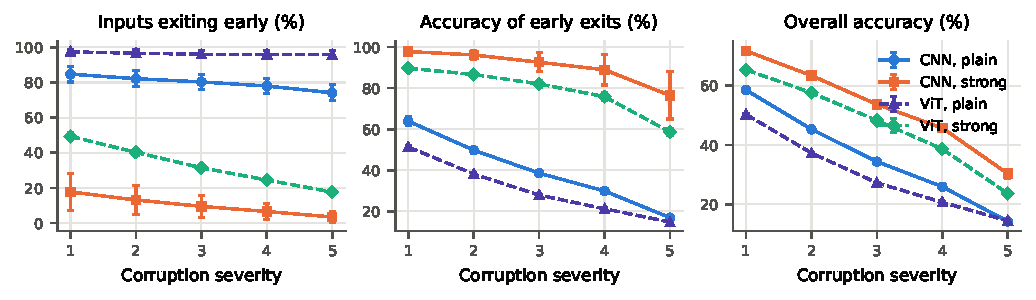
\includegraphics[width=\linewidth]{figures/two_by_two.pdf}
\caption{Architecture $\times$ recipe ($\alpha=0.5$, mean $\pm$ std over three seeds, averaged over six
corruptions). Overconfident models (plain recipe) keep exiting early as accuracy collapses; underconfident models
(strong recipe) back off, whatever the backbone.}
\label{fig:twobytwo}
\end{figure}

\subsection{Self-distillation trades clean efficiency for reliability}\label{sec:distill}
Distilling the final exit into the early ones strengthens them (exit-1 accuracy \cnncefirst\% at $\alpha=0$ against
\cnnkdfirst\% at $\alpha=0.5$) and makes routing cheaper on clean data (\cnncecost{} to \cnnkdcost{} GFLOPs at the
strict point). It also makes the exits more confident: at severity 5, the share of inputs exiting early rises from
\cnnceearly\% to \cnnkdearly\% and their accuracy falls from \cnnceprec\% to \cnnkdprec\%. The confidence gap of
exit 1 (mean confidence minus accuracy) at severity 5 grows from \cnncegap{} to \cnnkdgap{} points. The same
direction holds for the ViT trained with the strong recipe (early exits \vitceearly\% to \vitkdearly\%, accuracy
\vitceprec\% to \vitkdprec\%), although its exits stay underconfident. Figure~\ref{fig:confidence} (middle and
right) shows the dose-response over $\alpha$.

This differs from the common view that self-distillation improves
calibration~\citep{zhang2020selfdistillation,yun2020cskd,kim2021pskd} and from SAFE-KD's report of better corruption
robustness~\citep{khazem2026safekd}. In our setting the teacher is the model's own final exit, which is itself
overconfident (temperature \cnnkdtfinal{} on clean data), and distillation pulls the early exits towards it: exit 1
already becomes worse calibrated on clean data (ECE \cnnceecefirst\% without and \cnnkdecefirst\% with
distillation), consistent with calibration transfer from teacher to student~\citep{hebbalaguppe2024calibrationtransfer}
and with the growing teacher confidence noted by \citet{phuong2019distillation}. SAFE-KD differs in using an EMA
teacher with decoupled distillation and reports corruption error rather than exit decisions or calibration under
shift.

\begin{figure}[t]
\centering
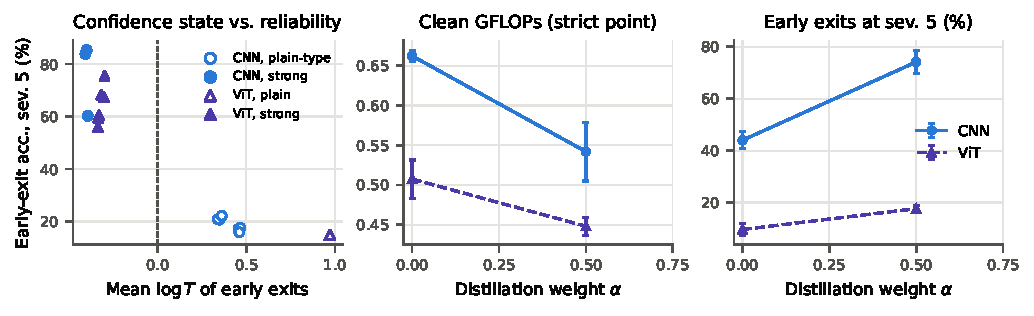
\includegraphics[width=\linewidth]{figures/confidence.pdf}
\caption{Left: confidence state of every run against the accuracy of early exits at severity 5 (filled: strong
recipe). Middle and right: distillation weight against clean cost at the strict point and the share of severely
corrupted inputs exiting early (mean $\pm$ std over seeds).}
\label{fig:confidence}
\end{figure}

\subsection{Clean calibration is mostly re-thresholding}\label{sec:calib}
Temperature scaling never changes predictions, and in practice it barely changes how an exit ranks inputs: the rank
correlation between raw and scaled confidence is at least \minrankcorr{} in every run, and the AUROC for separating
correct from incorrect predictions moves by at most 0.01 (Table~\ref{tab:calib}). With a single global threshold its
main effect is therefore to shift the effective threshold of each exit. \citet{kubaty2025rethinking} point out that
temperature scaling need not preserve rankings; in our models it nearly does. Tuning one threshold per exit directly on the
raw scores is cheaper than temperature scaling with a global threshold in every configuration, and for overconfident
models it is also cheaper than scaling with per-exit thresholds.

Under shift, temperatures fitted on clean data help overconfident models only partly and make underconfident models
worse calibrated (Table~\ref{tab:shift}), as \citet{ovadia2019trust} found for single-exit models. Applying
multi-domain temperature scaling~\citep{yu2022multidomain,gong2021confidence} per exit, with temperatures fitted on the
other corruption types (TS-LOCO), is far more effective for overconfident models: for the distilled CNN at severity 5, final-exit ECE falls from \cnnkdeceraw\%
(raw) and \cnnkdecets\% (clean TS) to \cnnkdeceloco\%, and the accuracy of early exits rises from \cnnkdprec\% to
\cnnkdprecloco\%, at the price of more computation on clean data (\cnnkdcost{} to \cnnkdcostloco{} GFLOPs at the
strict point).

\begin{table}[t]
\centering\small
\caption{Temperature scaling (TS) barely re-ranks inputs ($\rho_s$: rank correlation of raw and scaled confidence;
AUROC of confidence for correctness, raw / TS), and per-exit thresholds on raw scores beat a global threshold after
TS.}
\label{tab:calib}
\resizebox{\linewidth}{!}{\begin{tabular}{lrrrrrr}
\toprule
 & \multicolumn{2}{c}{Exit 1, raw vs.\ TS} & \multicolumn{4}{c}{Clean GFLOPs at the strict point} \\
\cmidrule(lr){2-3}\cmidrule(lr){4-7}
Configuration & $\rho_s$ & AUROC & Raw, global & Raw, per-exit & TS, global & TS, per-exit \\
\midrule
CNN, plain, $\alpha$=0 & 0.995 & 0.849 / 0.849 & 0.66\,$\pm$\,0.01 & 0.61\,$\pm$\,0.01 & 0.72\,$\pm$\,0.05 & 0.65\,$\pm$\,0.04 \\
CNN, plain, $\alpha$=0.5 & 0.991 & 0.845 / 0.844 & 0.54\,$\pm$\,0.04 & 0.50\,$\pm$\,0.01 & 0.61\,$\pm$\,0.07 & 0.55\,$\pm$\,0.02 \\
CNN, strong & 0.985 & 0.832 / 0.843 & 1.05\,$\pm$\,0.08 & 0.88\,$\pm$\,0.04 & 1.07\,$\pm$\,0.13 & 0.83\,$\pm$\,0.02 \\
ViT, plain & 0.956 & 0.828 / 0.838 & 0.20\,$\pm$\,0.01 & 0.20\,$\pm$\,0.01 & 0.29\,$\pm$\,0.11 & 0.24\,$\pm$\,0.06 \\
ViT, strong, $\alpha$=0 & 0.991 & 0.843 / 0.849 & 0.51\,$\pm$\,0.02 & 0.43\,$\pm$\,0.05 & 0.49\,$\pm$\,0.03 & 0.38\,$\pm$\,0.02 \\
ViT, strong & 0.987 & 0.836 / 0.844 & 0.45\,$\pm$\,0.01 & 0.37\,$\pm$\,0.03 & 0.42\,$\pm$\,0.01 & 0.34\,$\pm$\,0.03 \\
\bottomrule
\end{tabular}
}
\end{table}

\begin{table}[t]
\centering\small
\caption{Calibration under shift. TS uses temperatures fitted on clean validation data; TS-LOCO pools clean
validation data with the five other corruption types. Last column: clean GFLOPs at the strict point, raw / TS-LOCO.}
\label{tab:shift}
\resizebox{\linewidth}{!}{\begin{tabular}{lrrrrrrr}
\toprule
 & \multicolumn{3}{c}{Early-exit acc., sev.\ 5 (\%)} & \multicolumn{3}{c}{Final-exit ECE, sev.\ 5 (\%)} & Clean \\
\cmidrule(lr){2-4}\cmidrule(lr){5-7}
Configuration & Raw & TS & TS-LOCO & Raw & TS & TS-LOCO & GFLOPs \\
\midrule
CNN, plain, $\alpha$=0 & 21\,$\pm$\,1 & 27\,$\pm$\,3 & 37\,$\pm$\,2 & 58\,$\pm$\,2 & 37\,$\pm$\,2 & 16\,$\pm$\,1 & 0.66 / -- \\
CNN, plain, $\alpha$=0.5 & 17\,$\pm$\,1 & 21\,$\pm$\,2 & 26\,$\pm$\,3 & 62\,$\pm$\,1 & 40\,$\pm$\,1 & 18\,$\pm$\,0 & 0.54 / -- \\
CNN, strong & 76\,$\pm$\,11 & 74\,$\pm$\,19 & 76\,$\pm$\,12 & 15\,$\pm$\,3 & 32\,$\pm$\,2 & 18\,$\pm$\,2 & 1.05 / -- \\
ViT, plain & 15\,$\pm$\,0 & 20\,$\pm$\,7 & 22\,$\pm$\,9 & 62\,$\pm$\,0 & 26\,$\pm$\,1 & 12\,$\pm$\,0 & 0.20 / -- \\
ViT, strong, $\alpha$=0 & 70\,$\pm$\,4 & 67\,$\pm$\,6 & 70\,$\pm$\,5 & 11\,$\pm$\,0 & 23\,$\pm$\,0 & 16\,$\pm$\,0 & 0.51 / -- \\
ViT, strong & 59\,$\pm$\,2 & 54\,$\pm$\,3 & 59\,$\pm$\,1 & 11\,$\pm$\,0 & 24\,$\pm$\,0 & 16\,$\pm$\,0 & 0.45 / -- \\
\bottomrule
\end{tabular}
}
\end{table}

\section{Discussion and limitations}
Our recipe-over-architecture result concerns small models trained from scratch; for large pretrained models,
architecture strongly affects calibration~\citep{minderer2021revisiting}, and the two effects may interact. The
mechanism behind it, that soft-label regularisation lowers confidence, is known for single-exit
models~\citep{muller2019labelsmoothing,thulasidasan2019mixup,wang2023pitfall}; what our study adds is its consequence
for routing decisions. Early exits are often tuned for clean efficiency, and the choices that maximise it (distillation, little
regularisation) produce confident exits that are the least reliable when inputs drift. Choices that make exits
underconfident (label smoothing, mixup, strong augmentation) make exit decisions safer under shift but cost
efficiency at a strict accuracy target. Calibration fitted only on clean data does not resolve this trade-off,
whereas calibration fitted on diverse shifts does, which suggests calibrating exits on a mixture of anticipated
shifts when early-exit models are deployed in changing conditions. Our study is limited to CIFAR-100 at $32\times32$
resolution, one CNN and one transformer trained from scratch, six synthetic corruption types and three seeds per
configuration; component ablations use a single seed. TS-LOCO uses labelled corrupted data from other corruption
types, which is available only when such shifts can be simulated.

\section{Conclusion}
The reliability of early-exit decisions under distribution shift is governed by how confident the exits are, and
that confidence is set by the training recipe and by distillation rather than by the architecture. Confident exits
are cheap but brittle; underconfident exits are careful but costly. Exit confidence should be measured and chosen
deliberately, and calibrated on shifted data when early-exit models face changing inputs.

\bibliographystyle{plainnat}
\bibliography{refs}
\end{document}
